\documentclass[10pt,twocolumn,letterpaper]{article}
\usepackage[letterpaper,textwidth=7in,textheight=9in,centering]{geometry}
\usepackage{newtxtext,newtxmath}
\usepackage{graphicx,booktabs,amsmath,microtype,url,array}
\usepackage[colorlinks=true,urlcolor=blue,citecolor=black,linkcolor=black]{hyperref}
\usepackage[font=small,labelfont=bf]{caption}
\setlength{\columnsep}{0.25in}
\setlength{\parskip}{0pt}
\setlength{\textfloatsep}{7pt}
\clubpenalty=10000
\widowpenalty=10000
\brokenpenalty=10000
\makeatletter
\renewcommand\section{\@startsection{section}{1}{0pt}{8pt plus 2pt minus 1pt}{4pt}{\normalfont\fontsize{11}{12}\bfseries}}
\renewcommand\paragraph{\@startsection{paragraph}{4}{0pt}{5pt}{-0.7em}{\normalfont\normalsize\bfseries}}
\makeatother
\renewenvironment{abstract}{\noindent\textbf{Abstract.}\ }{\par\vspace{3pt}}
\newcommand{\ThirdAuthor}{Haodi Yuan}
\newcommand{\ThirdEmail}{\texttt{hay101@ucsd.edu}}
\newcommand{\sg}{\textsc{StateGuard}}
\title{\vspace{-1.7em}\sg: Failure Propagation and State-Consistent Recovery\\in Tool-Using Multi-Agent Workflows\vspace{-0.6em}}
\author{Xinying Liu\quad Jingwen Zhang\quad\ThirdAuthor\\
\small University of California San Diego, CSE 291A --- Option 5\\
\small \texttt{xil277@ucsd.edu}\quad\texttt{jiz333@ucsd.edu}\quad\ThirdEmail}
\date{}
\begin{document}
\fontsize{10}{12}\selectfont
\maketitle
\vspace{-2.5em}
\begin{abstract}
\sg{} studies failure propagation and state-consistent recovery in a tool-using deployment workflow. We implement a versioned runtime and record 99 real-model clean/fault pairs on AWS. Among 30 case/seed combinations valid under all three policies, task completion is 30\% without recovery, 100\% after full restart, and 80\% with verification. Restart approximately doubles tokens and latency on this workload. These Phase 1 measurements establish baselines for a later selective-recovery comparison.
\end{abstract}
\vspace{-0.5em}
\section{Research question and workflow}
An incorrect port can propagate from analysis into a plan and committed configuration. Replanning leaves the write behind; snapshot rollback may erase a later administrator update. Our questions are: \textbf{RQ1}, which message and state dependencies carry failures; \textbf{RQ2}, which work remains reusable after legitimate updates; and \textbf{RQ3}, when does selective recovery save more than its bookkeeping costs?

Consider a stale claim that an obsolete database port is valid. If the Planner acts on it, the Executor can commit an invalid API configuration while a worker scales independently and an administrator changes API replicas. Recovery must repair the port, preserve valid later writes, and recheck the shared CPU budget. The workload records result delivery, Planner consumption, and committed tool effects separately; a received message alone is not proof of propagation.

Config, Dependency, and Resource Agents analyze configuration, versioned knowledge, and capacity. A Planner consumes structured results; a controlled Executor modifies API, worker, and database state. Checkers enforce compatibility, resource budgets, deployment goals, and protected authentication/audit fields. Python, Pydantic, SQLite, a CLI runner, and pytest implement the system. A TritonAI adapter logs prompts, responses, tokens, timing, and retries; deterministic agents isolate runtime semantics.

\section{State-consistent recovery design}
The store maintains $S(k)=(x_k,v_k)$ for each field. Results carry parent IDs and read sets $R_r=\{(k,v)\}$. A typed graph connects results, actions, state versions, and external events through consumption, reads, triggers, and writes. Recording is automatic; Planner dependencies conservatively include all three analysis results rather than claiming exact semantic use.

Given faulty result $f$, invalidate $I(f)=\{f\}\cup\mathrm{Desc}(f)$. Reuse requires
\begin{equation}
r\notin I(f)\ \land\ \forall(k,v)\in R_r:\ v_k^{\mathrm{current}}=v.
\end{equation}
Missing provenance, tool effects, and resource constraints require further checks. Invalid analyses and the Planner are recomputed; eligible independent results are retained.

Writes carry an expected version and action ID. A SQLite transaction checks the version and commits state, ledger, and events together; identical retries return the recorded outcome after a simulated lost acknowledgement. Selective replay writes changed fields and blocks conflicting updates. Full restart rebuilds state and replays recorded external events in order with value/version preconditions. Irreversible effects remain explicit. Correct recovery requires task goals, invariants, preserved legitimate updates, and no new unauthorized effects. Local transactions do not guarantee rollback or exactly-once effects at remote services.

For a write to field $k$, the tool admits the action only when its supplied expected version equals the current $v_k$. An administrator write to that field invalidates the stale precondition; a write to an unrelated field need not. The final checker re-evaluates global constraints, so independent work is not automatically safe when it consumes a shared CPU budget. We classify a recovery as blocked or partial when a conflict or irreversible effect prevents the full objective.

The integrated suite passes \textbf{156 tests}, covering independent-result reuse, administrator updates, same-field conflicts, replay preconditions, and lost-ACK deduplication. Selective recovery is implemented and tested; its real-model comparison remains Phase 2 work.

\begin{figure*}[t]
\centering
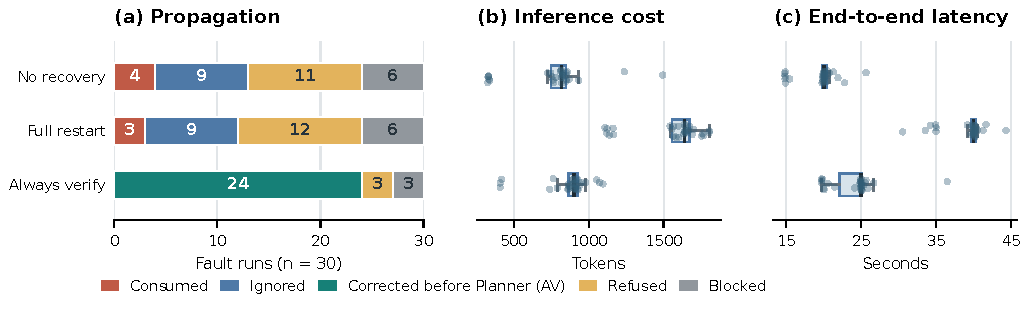
\includegraphics[width=\textwidth]{figures/propagation-cost.pdf}
\caption{Matched fault runs ($n=30$/policy). (a) Verdict after AV verification but before FR restart. (b--c) Fault-side tokens and latency include retries, restart, and pacing. Dots are runs; boxes show median/IQR.}
\label{fig:propagation-cost}
\end{figure*}

\section{Phase 1 experimental protocol}
\textbf{Baselines.} No recovery (NR) continues the injected workflow. Full restart (FR) executes a fresh clean attempt. Always verify (AV) checks intermediate outputs against simulated truth with one retry. AV is an optimistic oracle, not an independent detector. Recovery receives harness-supplied fault information, separating detection from recovery.

\textbf{Configuration.} The model is TritonAI \texttt{api-glm-5.3-flash}, called from an AWS CPU instance with Python 3.12.3. Each API request allows three attempts, with a five-second minimum request interval. Temperature is unspecified (provider default); seed labels 7, 11, and 19 fix fault schedules, not model sampling. Source revision is \texttt{6930ac8}. Each pair has clean/fault runs; FR adds a restart. Manifests and paired traces retain configuration, outputs, and failures.

\textbf{Workload.} One deployment task and topology exercise 11 cases: three wrong-port variants, two stale-protocol variants, two analysis timeouts, two malicious protected-field instructions, and two intended ignored controls. Thus $11\times3\times3=99$ pairs span the three policies. Earlier eight-scenario smoke and paired pilots are separate because retry settings differ. Lost ACK and external-update recovery are tested deterministically, not exercised by this real-model matrix.

\section{Measured results and failure analysis}
We record whether the injected result was exposed to a downstream agent, whether its content was consumed, and whether a bad action committed. An ignored instruction therefore contributes to the verdict distribution but cannot establish that a recovery algorithm repaired a propagated fault. Clean/fault pairs share a workload and injection schedule; model sampling remains uncontrolled across separate calls.

Of 99 recorded pairs, 96 are valid: two FR pairs (seed 7) have HTTP 422 errors; one NR pair (seed 19) fails its clean control without an API error. Excluding these combinations from \emph{every} policy leaves $9+11+10=30$ matched comparisons. Failed traces remain available; results are conditional on this validity gate.

\begin{table}[h]
\centering\small
\caption{Matched fault-side outcomes. Recomputed stages exclude AV verification retries; calls, tokens, and latency include retries and FR restart.}
\begin{tabular}{lrrr}\toprule
Metric & NR & FR & AV\\\midrule
Completed tasks & 9/30 & 30/30 & 24/30\\
Unauthorized commits & 0 & 0 & 0\\
Mean tokens & 756.7 & 1553.8 & 859.8\\
Mean latency (s) & 19.46 & 39.04 & 24.19\\
Mean model calls & 3.8 & 7.8 & 4.8\\
Mean recomputed stages & 0 & 4 & 0\\\bottomrule
\end{tabular}
\label{tab:results}
\end{table}

FR completes all matched tasks at $2.05\times$ NR's tokens and $2.01\times$ its latency. AV reaches 80\% completion at $1.14\times$ the tokens and $1.24\times$ the latency. Figure~\ref{fig:propagation-cost} shows the per-run distributions; latency includes pacing, not just model compute.

NR has 4 consumed, 9 ignored, 11 refused, and 6 blocked injections. Under AV, the 24 raw ``ignored'' verdicts all follow a failed verification and a valid retry; the faulty outputs never reach Planner. Figure~\ref{fig:propagation-cost} therefore labels these \emph{corrected before Planner}, retaining the raw verdicts in the traces. Under NR, all six adversarial runs succeed because the model ignores the injected instructions. Zero unauthorized commits does not establish recovery from an accepted attack.

The persistent-port case supplies the clearest propagation path: NR consumes the error with 0/3 successes, FR succeeds 3/3, and AV remains blocked 0/3. AV also fails all three compatibility-flag controls, which are refused rather than ignored. Among accidental cases, completion is 3/24, 24/24, and 18/24 for NR, FR, and AV. Aggregate scores therefore conceal systematic case-level failures.

\section{Remaining proposal and evaluation plan}
This pilot covers one task/topology and constrained tools. Detection, tracking overhead, and selective-recovery performance remain unevaluated. Phase 2 will compare dependency-only and state-aware replay against FR and AV under identical fault identities, event schedules, and budgets. We target 24--36 tasks, adjusted after a cost pilot, with chain, fan-out, and diamond dependencies; unchanged state, unrelated updates, same-field conflicts, and shared-resource contention. We will separate development and evaluation workloads.

\clearpage
\section*{Appendix: Architecture and milestones}
\vspace{-0.5em}
\noindent\begin{minipage}{\columnwidth}
\centering
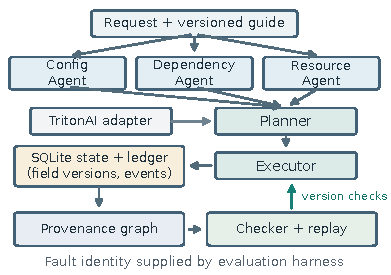
\includegraphics[width=.96\columnwidth]{figures/architecture.pdf}
\captionof{figure}{StateGuard runtime. A shared TritonAI adapter serves analysis agents and Planner; the runtime records versioned writes and provenance. Recovery checks a known faulty result before replay or blocking.}
\label{fig:architecture}
\end{minipage}
\par\vspace{0.8em}
\noindent\begin{minipage}{\columnwidth}
\centering
\captionof{table}{Project milestones (2026).}
\begin{tabular}{@{}p{1.05in}>{\raggedright\arraybackslash}p{2.01in}@{}}\toprule
When & Deliverable and acceptance check\\\midrule
Nov. 3--15 & Freeze artifacts; expand graph and event cases.\\
Nov. 16--25 & Compare replay methods on matched faults.\\
Nov. 26--Dec. 4 & Measure precision, conflicts, cost, and overhead.\\
\mbox{Dec.~5--10} & Reproduce results; submit code and final report.\\\bottomrule
\end{tabular}
\label{tab:milestones}
\end{minipage}

\paragraph{Evidence boundary.}
Manifests, paired traces, checker outcomes, and analysis scripts reproduce the matched figures. The 156-test suite exercises controlled replay; the real-model matrix measures NR, FR, and AV. Detection, selective-replay performance, and arbitrary remote effects remain unmeasured.

\paragraph{Phase 2 evaluation.}
Chain, fan-out, and diamond workloads will test external updates and shared-state conflicts. Ablations remove field reads, version checks, and action deduplication. We will measure invalidation precision/recall, preserved work, blocked effects, tokens, latency, and tracking overhead.

\paragraph{Related work.}
AgentDojo~\cite{agentdojo}, TAMAS~\cite{tamas}, and A2ASecBench~\cite{a2a} evaluate agent security; our traces additionally connect faulty outputs to state writes. RDD lineage~\cite{rdd} and lineage-driven fault injection~\cite{ldfi} motivate causal slices, while Falkirk Wheel~\cite{falkirk} studies selective rollback. Optimistic concurrency control~\cite{occ} informs conditional writes. Sagas~\cite{sagas} and rollback-recovery protocols~\cite{rollback} make clear why external effects need explicit treatment.

\paragraph{Validity and artifacts.}
AV reads simulated truth, so it is an oracle baseline. Seeds fix injection schedules, not provider sampling; results cover one task, topology, model, and pacing rule. Controlled-tool tests do not establish guarantees for remote services. Code and traces are in the \href{https://github.com/ashley-tech628/CSE291A-StateGuard}{artifact repository}.

\begin{thebibliography}{9}\setlength{\itemsep}{0pt}\small
\bibitem{agentdojo} E. Debenedetti et al. AgentDojo: A dynamic environment to evaluate prompt injection attacks and defenses for LLM agents. \emph{arXiv:2406.13352}, 2024.
\bibitem{tamas} I. Kavathekar et al. TAMAS: Benchmarking adversarial risks in multi-agent LLM systems. \emph{ACL}, 2026.
\bibitem{a2a} T. Li et al. A2ASecBench: A protocol-aware security benchmark for agent-to-agent multi-agent systems. \emph{ICLR}, 2026.
\bibitem{rdd} M. Zaharia et al. Resilient distributed datasets: A fault-tolerant abstraction for in-memory cluster computing. \emph{NSDI}, 2012.
\bibitem{ldfi} P. Alvaro, J. Rosen, and J. M. Hellerstein. Lineage-driven fault injection. \emph{SIGMOD}, pp. 331--346, 2015.
\bibitem{falkirk} M. Isard and M. Abadi. Falkirk Wheel: Rollback recovery for dataflow systems. \emph{arXiv:1503.08877}, 2015.
\bibitem{occ} H. T. Kung and J. T. Robinson. On optimistic methods for concurrency control. \emph{ACM TODS} 6(2):213--226, 1981.
\bibitem{sagas} H. Garcia-Molina and K. Salem. Sagas. \emph{SIGMOD}, 1987.
\bibitem{rollback} E. N. Elnozahy et al. A survey of rollback-recovery protocols in message-passing systems. \emph{ACM Computing Surveys} 34(3):375--408, 2002.
\end{thebibliography}
\end{document}
